%%%%%%%%%%%%%%%%%%%%%%%%%%%%%%%%%%%%%%%%%%%%%%%%%%%%%%%%%%%%%%%%
% Sablona pro zaverecnou zpravu k semestralni praci z BI-ZUM
% Kódování dokumentu: UTF8
% Verze: 1.0 (2013-01-28)
% Autor: Ing. Martin Šlapák
%%%%%%%%%%%%%%%%%%%%%%%%%%%%%%%%%%%%%%%%%%%%%%%%%%%%%%%%%%%%%%%%
%
% NEUPRAVUJTE PROSIM PARAMETRY DOKUMENTU, JAKO OKRAJE CI PISMO!
%
%%%%%%%%%%%%%%%%%%%%%%%%%%%%%%%%%%%%%%%%%%%%%%%%%%%%%%%%%%%%%%%%
%
% Celkova delka zpravy nesmi presahnout 1 stranu A4, vyjadrujte 
% se strucne, jasne a vecne - zadne omacky a slovni vata. Diky!
% Neprehazujte ani poradi sekci.
%
%%%%%%%%%%%%%%%%%%%%%%%%%%%%%%%%%%%%%%%%%%%%%%%%%%%%%%%%%%%%%%%%
\documentclass[a4paper,10pt,twocolumn]{article}
\usepackage{lmodern}
\usepackage[czech]{babel}
\usepackage[T1]{fontenc}
\usepackage[utf8]{inputenc}
\usepackage{graphicx}
\usepackage{float}
\usepackage[top=0.5cm,bottom=2cm,left=1cm,right=1cm]{geometry}
%gobble sezere cisla stranek, takze nebudou zadna
\pagenumbering{gobble} 
\title{Zpráva k 4. domácímu úkolu z předmětu MI-PAA}
\date{\today}
%%%%%%%%%%%%%%%%%%%%%%%%%%%%%%%%%%%%%%%%%%%%%%%%%%%%%%%%%%%%%%%%
% tady nastavte své jméno a email
\author{Jan Sokol \\ sokolja2@fit.cvut.cz}
%%%%%%%%%%%%%%%%%%%%%%%%%%%%%%%%%%%%%%%%%%%%%%%%%%%%%%%%%%%%%%%%
\begin{document}
\maketitle
%%%%%%%%%%%%%%%%%%%%%%%%%%%%%%%%%%%%%%%%%%%%%%%%%%%%%%%%%%%%%%%%
\begin{abstract}

Zvolte si heuristiku, kterou budete řešit problém vážené splnitelnosti booleovské formule (simulované ochlazování, simulovaná evoluce, tabu prohledávání). \\
Tuto heuristiku použijte pro řešení problému batohu. Můžete použít dostupné instance problému, anebo si vygenerujte své instance pomocí generátoru. Používejte instance s větším počtem věcí (>30). \\
Hlavním cílem domácí práce je seznámit se s danou heuristikou, zejména se způsobem, jakým se nastavují její parametry (rozvrh ochlazování, selekční tlak, tabu lhůta…) a modifikace (zjištění počáteční teploty, mechanismus slekce, tabu atributy…). Není-li Vám cokoli jasné, prosíme ptejte se na cvičeních. \\
Problém batohu není příliš obtížný, většinou budete mít k dispozici globální maxima (exaktní řešení) z předchozích prací, například z dynamického programování. Závěrečná úloha je co do nastavení a požadovaného výkonu heuristiky podstatně náročnější a může vyžadovat zcela jiné nastavení parametrů.


% Zde shrňte v několika větách co jste dělali, jak jste to dělali, jakých výsledků jste dosáhli. Vypíchněte to nejzajímavější. Zkusili jste nějakou pokročilou techniku? Tady se s ní pochlubte a pak ji dále rozepište v patřičné sekci. Zkuste se vejít do 150 slov.
\end{abstract}

%%%%%%%%%%%%%%%%%%%%%%%%%%%%%%%%%%%%%%%%%%%%%%%%%%%%%%%%%%%%%%%%
\section{Výběr jazyka}
Pro svou implementaci problému batohu jsem si vybral jazyk Python. Ačkoli to je jazyk interpretovaný a nečekal jsem závratné rychlosti výpočtů, mojím výběrem byl pro to, že jsem jazyk znal a pro jakýkolik koncept je pro mne nejrychlejší.


\section{Testovací Hardware}
Všechny testy byly prováděny na cloudové linuxové instanci v AWS, běžící na Red Hat Enterprise Linux 7. Velikost instance byla:
  2 Core CPU / 8 GB RAM, v názvosloví AWS \textbf{m4.large}.


\section{Měření výpočetního času}
Výpočet běhu funkce je řešen tak, že je spočten strojový čas před během funkce, a také po něm. Tyto časy jsou od sebe odečteny a je vrácen čas v ms.

   \begin{verbatim}
def timing(f):
    def wrap(*args):
        time1 = time.time()
        ret = f(*args)
        time2 = time.time()
        measured_time.append(
          {'type': f.__name__,
           'time': (time2-time1)*1000.0})
        return ret
    return wrap
   \end{verbatim}


\subsection{Popis algoritmu}

Zde uvádím úryvek kódu řídící evoluci. Celý funkční kód je k dispozici v repozitáři.

Nejdříve vytvoříme počáteční populaci. Potom v n generacích běžíme nasledovné:
\begin{itemize}
  \item vytřídíme nejlepší jedince dle fitness funkce necháme je soupeřit v turnaji,
  \item dle nastaveného elitismu převezmeme x jedinců z minulého kola do tohoto,
  \item vyplníme novou generaci novými jedinci, kteří jsou:
\begin{itemize}

  \item kříženci dvou náhodných minulých jedinců,
  \item nebo jeden náhodný jedinec.
\end{verbatim}
  \item mutujeme náhodné bity těchto nových jedinců
  \item ověříme, zda jedinec je validní (náklad batohu je menší, než je jeho kapacita).

\end{verbatim}

   \begin{verbatim}

# Create initial population
population = create_population(self.population_size,
                                    size)

# Run n generations
for generation in range(0, self.generations):
  sorted_population = sort_population(population)

  # Selection
  new_population = self.tournament(population,
                       self.tournament_count, 
                       self.tournament_pool_size )

  # Elitsm
  del sorted_population[self.elitism_count:]

  new_population.extend(sorted_population)
  sorted_population = sort_population(new_population)

  # Fill population with new children
  while len(new_population) != self.population_size:
      child = []
      # Crossover
      if odds_are(self.xover_probability):
          in1 = self.random_individual(new_population)
          in2 = self.random_individual(new_population)

          child = self.crossover_single(in1, in2)
      else:
          # Just pick random individual
          child = deepcopy(random_individual(population))

      # Mutation
      child = self.mutator_random_inverse(child,
                           self.mutation_probability)

      # Check if mutated/crossed individual is valid
      if self.constraint_fn(child):
          new_population.append(child)
   \end{verbatim}





\subsection{Experimenty s nastavením parametrů}


Různě jsem nastavoval parametry genetického algoritmu - pravděpodobnost křížení, pravděpodobnost mutace, elitismus, velikost turnaje, počet turnajů a počet generací. Z grafů jsem poté usoudil, které hodnoty jednotlivých parametrů jsou nejlepší.


\subsection{Pravděpodobnost křížení}

Osobně hodnotím 0.3 až 0.4 jako nejlepší hodnotu pravděpodobnosti křížení. Při pravděpodobnosti 0.7 a více ani nebylo možné dosáhnout optimální hodnoty.

\begin{figure}[H]
  \begin{center}
    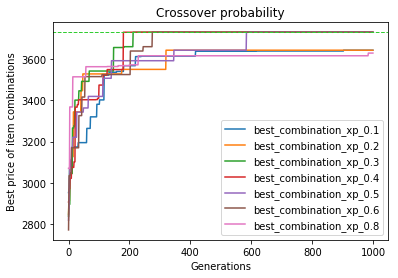
\includegraphics[height=6cm]{graphs/xover_probability.png}
  \end{center}
  % \caption{Graf vývoje fitness}\label{fig1}
\end{figure}

\subsection{Pravděpodobnost mutace}


Na grafu velmi dobře vidíme, že tato hodnota by měla být nízká.
Osobně hodnotím 0.025 až 0.1 jako nejlepší hodnotu pravděpodobnosti mutace. Při pravděpodobnosti 0.7 a více ani nebylo možné dosáhnout optimální hodnoty.

\begin{figure}[H]
  \begin{center}
    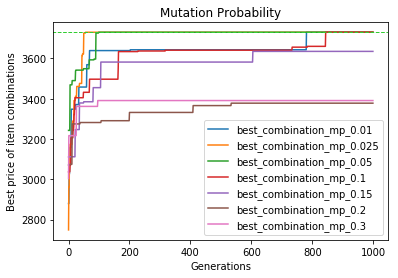
\includegraphics[height=6cm]{graphs/mutation_probability.png}
  \end{center}
  % \caption{Graf vývoje fitness}\label{fig1}
\end{figure}


\subsection{Elitismus}

Vysoký elitismus zvýhodňuje kvalitnější jedince a znevýhodňuje slabší jedince, kteří ale v sobě mohou nést lepší informaci.

Pokud toto nastavíme na vysokou hodnotu, velmi často uvízneme v lokálním maximu/minimu.

Na grafu vidíme, že elitismus se zdá být nejlepší při hodnotě 5.


\begin{figure}[H]
  \begin{center}
    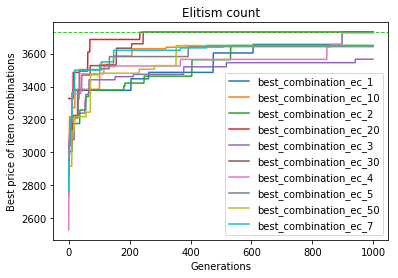
\includegraphics[height=6cm]{graphs/elitism_count.png}
  \end{center}
  % \caption{Graf vývoje fitness}\label{fig1}
\end{figure}


\subsection{Velikost turnaje}

Turnajem se vybírají jedinci ke křížení. Do každého turnaje vstupuje několik náhodných jedinců z celé populace.

Tento parametr se chová obdobně, jako elitimus, při velkých turnajích jsou znevýhodněni slabší jedinci.

Pokud toto nastavíme na vysokou hodnotu, velmi často uvízneme v lokálním maximu/minimu.

Na grafu vidíme, že velikost turnaje se zdá být nejlepší při hodnotě 2.


\begin{figure}[H]
  \begin{center}
    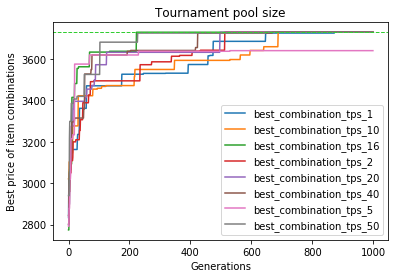
\includegraphics[height=6cm]{graphs/tournament_pool_size.png}
  \end{center}
  % \caption{Graf vývoje fitness}\label{fig1}
\end{figure}



\subsection{Počet turnajů}

Turnajem se vybírají jedinci ke křížení. Z každého turnaje je vybírán vždy jeden, tudíž počet turnajů nepřímo určuje, kolik jedinců bude vybráno ke křížení do nové populace.


Na grafu vidíme, že počet turnajů se zdá být nejlepší při hodnotě 20 až 50.



\begin{figure}[H]
  \begin{center}
    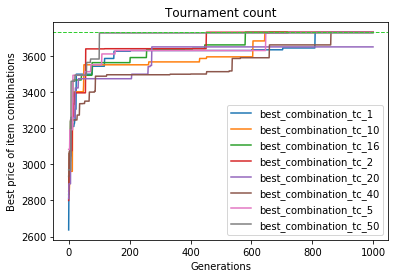
\includegraphics[height=6cm]{graphs/tournament_count.png}
  \end{center}
  % \caption{Graf vývoje fitness}\label{fig1}
\end{figure}


\subsection{Počet generací}

Počtem generací jsem zjišťoval, kolik nejméně generací je potřeba, dokud nedojde ke konvergenci, pro instance s 30 předměty.

Jako moment pro ukončení evoluce jsem vybral 1000 generací, ikdyž jak vidíme níže na grafu, tato hodnota má poměrně velkou rezervu.


\begin{figure}[H]
  \begin{center}
    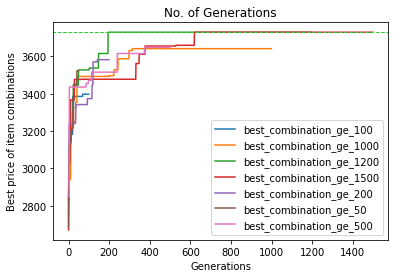
\includegraphics[height=6cm]{graphs/generations.png}
  \end{center}
  % \caption{Graf vývoje fitness}\label{fig1}
\end{figure}


\section{Shrnutí a závěr}

Pokročilá iterativní metoda je nesmírně efektivní při velkých počtech předmětů v instanci.

Přesnost se pohybuje kolem 90-100\% (tj, relativní chyba většinou menší, než 10\%) a čas strávený výpočtem je několikařádově menší, než při použití jiných metod.

Implementace byla úspěšná a napsána pro jednoduchou výměnu batůžku  na SAT. \\
Pro vytváření grafů bylo využito Python notebooku, který je přiložen v adresáři \textbf{report/}. Grafy jsou vykresleny pomocí knihovny \textbf{mathplotlib}.

% Tady okomentujte k čemu se váš evoluční algoritmus dopracoval, co se vám povedlo, co ne a jak by to šlo vylepšit. Jakého nejlepšího řešení se vám podařilo dosáhnout. Klidně i napište, co se vám na semestrální práci líbilo a taky co byste raději měli jinak. Uvítáme jakékoli nápady. 

% Pokud jste čerpali z nějaké literatury, měli byste ji řádně ocitovat.

% \textbf{A NEZAPOMEŇTE, ŽE SE MUSÍTE VEJÍT NA JEDNU A4! ;-)}

%%%%%%%%%%%%%%%%%%%%%%%%%%%%%%%%%%%%%%%%%%%%%%%%%%%%%%%%%%%%%%%%
% odtud dal to pak zakomentujte pomoci znaku procenta na zacatku radku
% \begin{center}
% \line(1,0){250}
% \end{center}

% \textbf{Pár poznámek pod čarou\ldots}
% \begin{itemize}
%   \item Zdroják této šablony je v kódování UTF8.
%   \item Neměňte prosím žádná nastavení dokumentu, okrajů, velikosti písma apod.
%   \item Nepřehazujte ani pořadí sekcí.
%   \item \textbf{Jak zprávu zkompilovat?} Použijte dvakrát (kvůli odkazům a referencím) tento příkaz:

%   \begin{verbatim}
%   pdflatex zdrojak-zpravy.tex
%   \end{verbatim}

%   Výsledkem bude \textbf{zdrojak-zpravy.pdf}. 

%   \item Pokud něco nepůjde, konzultujte na cvičeních BI-TED či se spolužáky. Cvičící BI-ZUM nebudou mít čas řešit detaily s {\LaTeX}em.
%   \item \textbf{Proč se sakra musím vejít na 1 A4?} Chceme, abyste si vyzkoušeli jak napsat to podstatné, vybrat to důležité, vyhnout se takové té textové vatě. Současně po vás nechceme psaní dlouhých esejí, raději svůj čas věnujte svým algoritmům. A taky, kdo má číst 5 stran napsaných \uv{protože to chtěj}. ;-)
%   \item TIP: Tuto zprávu může být reálné uplatnit i jako jeden z domácích úkolů na BI-TED. K tomu vás ale nenutíme a také počítejte s tím, že tam po vás mohou chtít další rozšíření dokumentu. \textbf{Ale zase: proč nezabít dvě mouchy jednou ranou?}
% \end{itemize}

\end{document}
